\documentclass{beamer}

%style
\mode<presentation>
\usetheme{Boadilla}

%Einstellungen der Präsentation
\title[Offensive Security]{Fuzzing Methods}
\subtitle{Offensive Security}
\author{Moritz Rupp}
\institute[MR]{Hochschule Albstadt-Sigmaringen}
\setbeamertemplate{navigation symbols}{}%remove navigation symbols
\date{SS 22}

%Beginn der Präsentation
\begin{document}
\begin{frame}
 \titlepage
\end{frame}
\begin{frame}{Contents}
 \tableofcontents
\end{frame}
\section{Fuzzing background}
\begin{frame}{Fuzzing background}
\begin{itemize}
 \item Development produces bugs, errors and unintentionally behaviour\\
 $\rightarrow$ Gateway for vulnabilities and exploits
 \item Software testing tries to oppose that
 \item Many different approaches exist
\end{itemize}
\end{frame}
\subsection{Software testing}
\begin{frame}{Software testing}
 \begin{block}{Manuel testing}
  - Code reviews, manuel search for vulnabilities\\
  - Time consuming, expensive
 \end{block}
\begin{block}{Static analysis}
- Automatically examine source code before the programm is run\\
- Pattern analysis \\
- Control flow graph, data flow analysis\\
- Expensive tooling
\end{block}
\begin{block}{Dynamic analysis}
- Automatically examine a programm while its's been run\\
- Execute and input data in real-time\\
\end{block}
\end{frame}
\subsection{Fuzz-testing}
\begin{frame}{Fuzz-testing}

  $\Rightarrow$ Fuzz-testing is the cutting edge of dynamic analysis
  
  \begin{itemize}
   \item Input forget data in real-time
   \item Monitor the system behaviour
   \item Listen for exceptions
   \item Provide feedback
  \end{itemize}

\end{frame}
\section{Functionality}
\begin{frame}{Functionality}
\begin{enumerate}
 \item Identify target interfaces\\
 $\rightarrow$ portscanning, code reviews
 \item Generate inputs\\
 $\rightarrow$ mutation, generation based fuzzing
 \item Feed these inputs to the target system
 \item Monitor for exceptions
 \item Log exceptions
\end{enumerate}

\end{frame}
\begin{frame}{Basic Fuzzing application}
\begin{center}
  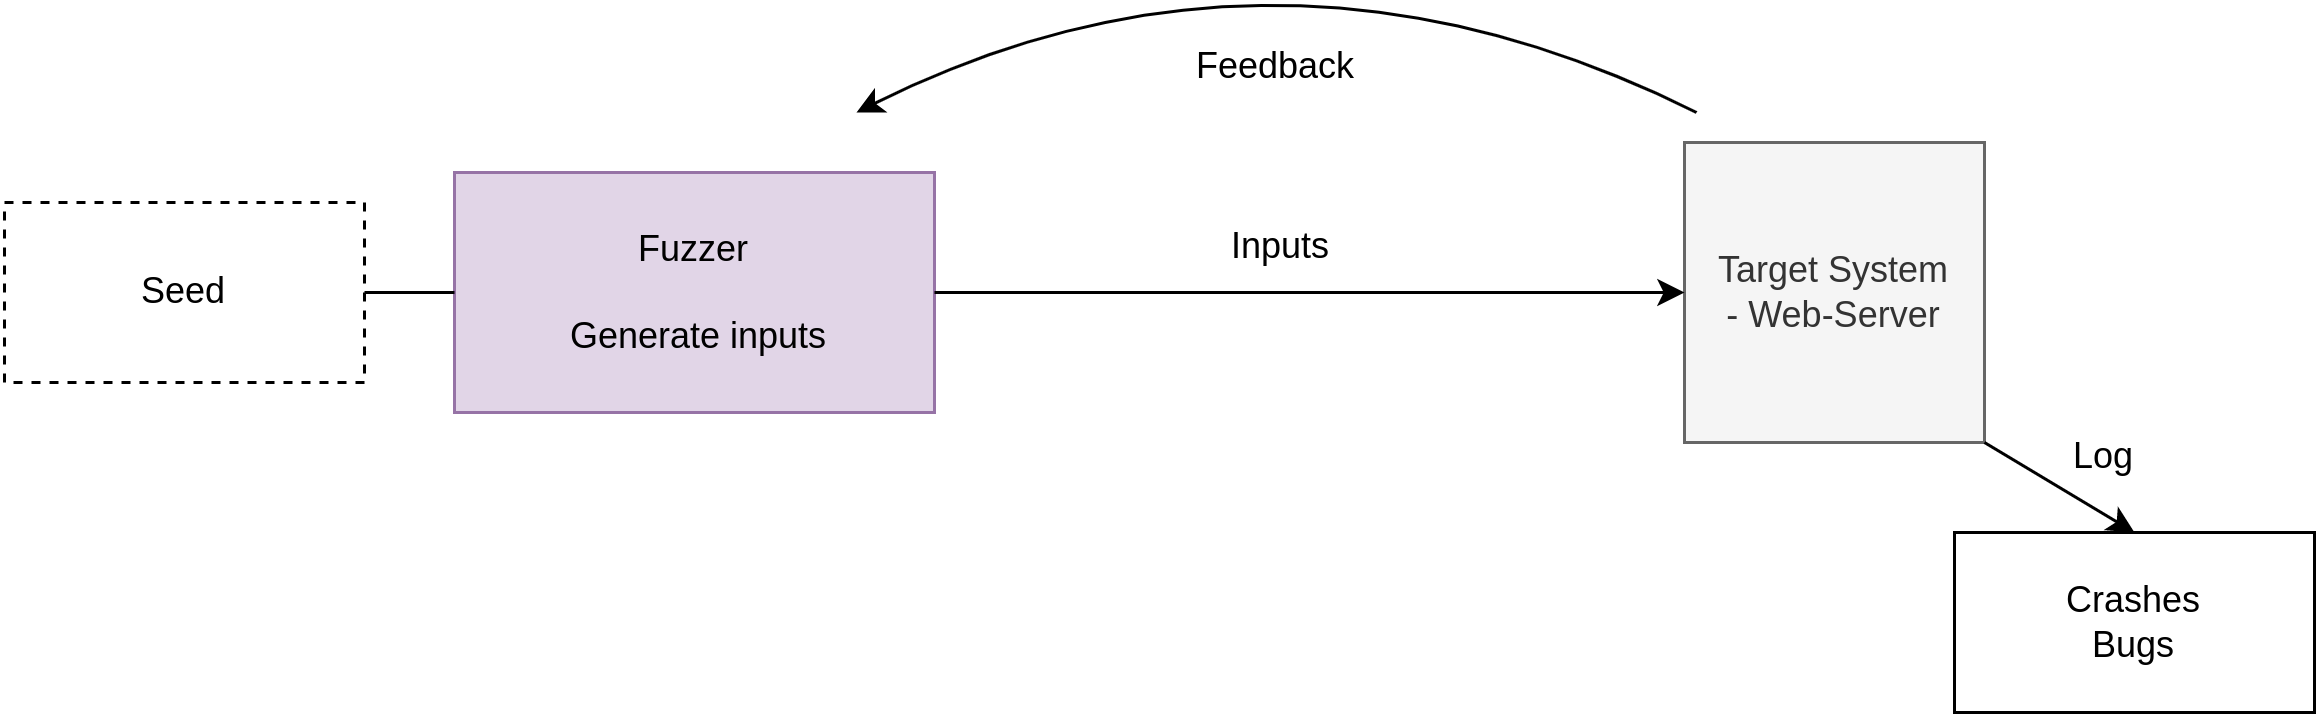
\includegraphics[scale=0.15]{basicfuzz.png}
\end{center}
\end{frame}
\section{Fuzzing Methods}
\begin{frame}{Fuzzing Methods}
 \begin{itemize}
  \item Huge landscape of applications and infrastructers\\
  $\rightarrow$ Web-applications, networks, binarys etc.\\
  $\Rightarrow$ No generall solution
  \item Different targets expect different inputs
  \item How do we generate those inputs?\\
  $\Rightarrow$ Random fuzzing\\
  $\Rightarrow$ Mutation based fuzzing\\
  $\Rightarrow$ Generation based fuzzing
 \end{itemize}

\end{frame}
\subsection{Random fuzzing}
\begin{frame}{Random Fuzzing}
 \begin{itemize}
 \item Earliest fuzzing approach
  \item Generate pseudo random values of a given seed
  \item Mostly usefull for black box testing\\
  $\rightarrow$ Closed source projects
    \item Will generate lots of rejected test-cases

 \end{itemize}

\end{frame}
\begin{frame}{Random based fuzzer}
\begin{center}
 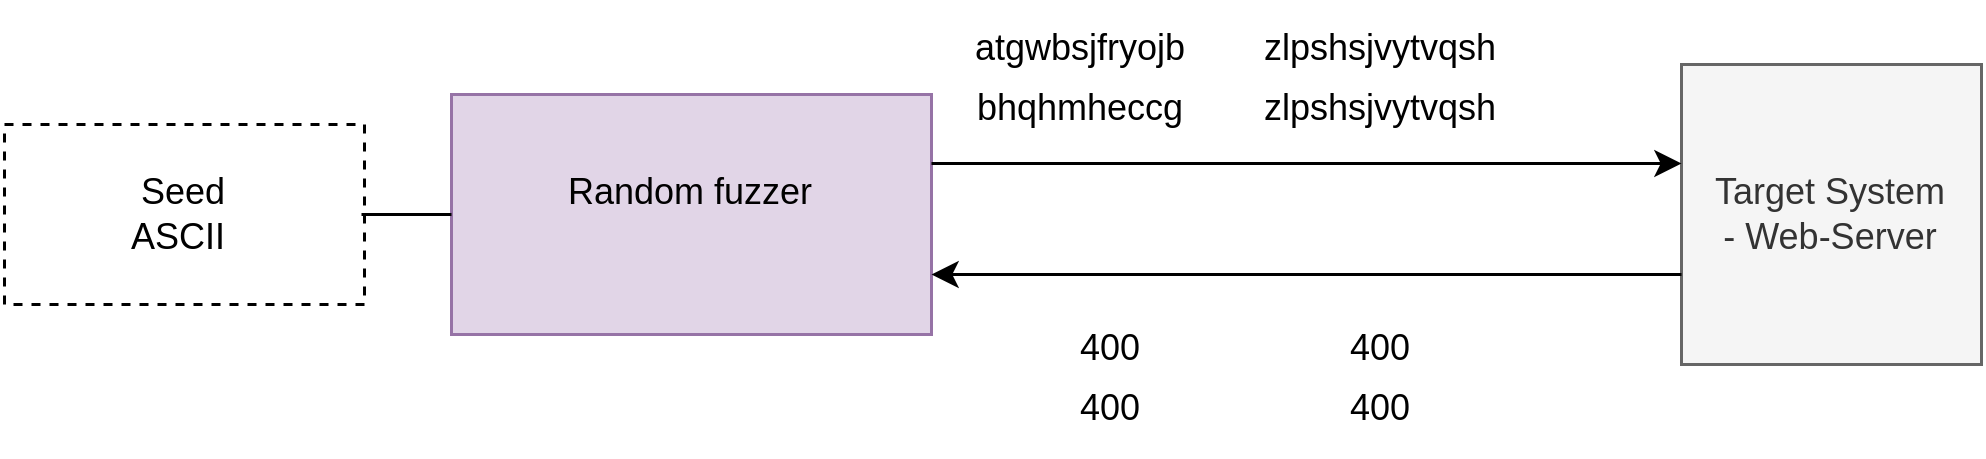
\includegraphics[scale=0.15]{basic2.png}
 \end{center}
 \end{frame}
\subsection{Mutation based fuzzing}
\begin{frame}{Mutation based Fuzzing}
\begin{itemize}
 \item Generate test-cases based on already existing data\\
 $\Rightarrow$ Record valid inputs\\
 $\Rightarrow$ Mutate these inputs
 \item Randomly or after fixed patterns
 \item No need for deep protocol knowledge
 \item Flip random nummber of bits
 
 
\end{itemize}
\end{frame}
\begin{frame}{Mutation based Fuzzer}
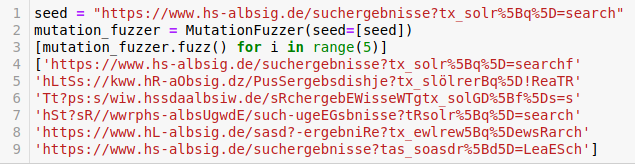
\includegraphics[scale=0.5]{mutatate.png}\footnote{Andreas Zeller}
\end{frame}
\begin{frame}
 \begin{itemize}
 \item Determine the seed correctly\\
 $\Rightarrow$ 'suchergebnisse?fuzz'
  \item Setup fixed grammars\\
  $\Rightarrow$ http/
  fuzz
 \end{itemize}
 
\end{frame}
\subsection{Generation based fuzzing}
\begin{frame}{Generation based Fuzzing}
 \begin{itemize}
  \item Generate inputs from scratch
  \item Based on the specification and format
  \item Protocol knowledge is importand
  \item Generated inputs are semi-valid
  \item Will barely generate rejected test-cases
  \item Have to be developed from scratch for every protocol/application 
  
 \end{itemize}
\end{frame}
\begin{frame}
 \begin{itemize}
   \item Assemple every part of an input sepperatly
   \item Assign rules to these indivual parts
  \end{itemize}
 
\end{frame}
\begin{frame}{Creation rules in Sully}
\begin{table}[]
\begin{tabular}{lllll}
s\_static  &  &  set a static value  \\
s\_string  &  &  fuzz the provided string  \\
s\_delim  &  &   fuzz delimters  \\
\end{tabular}
\end{table}
\end{frame}

\begin{frame}{Fuzzing of an http request}
 $\rightarrow$ GET /index.html HTTP \dots

\begin{center}

 \begin{table}[]
 \begin{tabular}{lllll}
 s\_static('GET')  &  &  &  \\
  s\_delim(' ')\\
 s\_delim('/')\\
    s\_string('index)\\
   s\_static('.')  &  \\
 s\_string('html')\\
 s\_delim(' ')\\
 s\_string('HTTP')&  &  & 
 \end{tabular}
 \end{table}
  
 \end{center}

\end{frame}
\section{Tooling}
\begin{frame}{Tooling}
 \begin{itemize}
  \item Fuzzing is almost always executed with tooling
  \item Manuel testing only usefull in rare cases
  \item Many different tools exist for different fuzzing methods/targets\\
  $\Rightarrow$ OSS-Fuzz, Wfuzz, Sully, FuzzDB \dots
 \end{itemize}

\end{frame}
\begin{frame}{AFL}
 $\Rightarrow$ American fuzzing loop
 \begin{itemize}
 \item Open-source
  \item Mutation and generation based Fuzzer
  \item Widely used across many target systems
  \item Responsible for lots of relevant findings\\
  $\rightarrow$ X.Org Server, PHP, OpenSSL, Firefox, bash \dots
 \end{itemize}

\end{frame}

\section{Practical example}

\begin{frame}{Practical example}
 
\end{frame}
\section{Conclusion}
\begin{frame}{Conclusion}
 \begin{itemize}
 \item Fuzzing effectively locates bugs\\
 $\rightarrow$ Mostly simple bugs
 \item Boosts stability and security of systems
  \item Quite complex
 \end{itemize}

\end{frame}
\begin{frame}{Quellen}
Li, J., Zhao, B. \& Zhang, C. Fuzzing: a survey. Cybersecur 1, 6 (2018). https://doi.org/10.1186/s42400-018-0002\-y\\
https://www.ionos.com/digitalguide/websites/web-development/what-is-fuzzing/

\end{frame}








\end{document}
